\newpage{\ } 
\thispagestyle{empty} 

\chapter{Pruebas experimentales}
\lhead{Cap\'itulo 5. \emph{Pruebas experimentales}} % This is for the header on each page - perhaps a shortened title
En este capítulo se menciona las m\'etricas de evaluaci\'on utilizadas para medir el desempe\~{n}o de la metodolog\'ia propuesta. Por otro lado, se detallan los experimentos realizados y los resultados de la metodolog\'ia propuesta, seguidamente se esboza la comparaci\'on y la posterior discusi\'on de los mismos.

\section{Caso de estudio}
Filadelfia es una ciudad de Paraguay, del departamento de Boquer\'on, del Chaco paraguayo(lat-long $22^{o}20^{,}00^{,,} S - 60^{o}01^{,} 00^{,,} O$ ) con una superficie de 13.879 $ km^{2} $. Fue elevada a nivel de distrito en 2006. Su poblaci\'on la constituyen principalmente colonos menonitas. Fundada junto a otras localidades menonitas a finales de la d'ecada de 1920, ha desarrollado una cultura espec\'ifica, transmitida a lo largo de los siglos a trav\'es de la religi\'on, y una infraestructura productiva que le aporta a sus residentes alto poder de compra. Estas comunidades menonitas trabajan con modernas t\'ecnicas de producci\'on agropecuaria, fabricaci\'on de productos l\'acteos y procesamiento de s\'esamo y man\'i. Pueden ser ubicadas dentro de las imagenes landsat con path-Row 228-76 y en las VCF con c\'odigo KJ1920.\\~\\
Se opto por esta localizaci\'on debido a que ademas de estar ubicada en el Chaco Paraguayo posee un crecimiento demogr\'afico en la que las actividades agr\'icolas y ganaderas son variantes, proporcionando un ambiente ideal para las distintas pruebas y validaciones necesarias.\\~\\

\section{Métricas de evaluación}
Para realizar el control de calidad, algunos se basan en el concepto de matriz de confusi\'on, que establece una relaci\'on entre los resultados obtenidos en el proceso de asignaci\'on y la informaci\'on verdad terreno $ (VT) $ disponible para la zona de estudio. La diagonal principal representa el n\'umero de celdas correctamente catalogadas $ (T) $ , y la diagonal transpuesta, las incorrectamente catalogadas $ (F) $ . El uso de esta matriz presenta como mayor desventaja que est\'a condicionada a la veracidad y exactitud de la referencia utilizada como $ VT $.

\begin{table}[H]
	\centering
\begin{tabular}{|
		>{\columncolor[HTML]{EFEFEF}}l |l|l|l|}
	\hline
	\textbf{Categorias}             & \cellcolor[HTML]{EFEFEF}\textbf{Perdida (VT)} & \cellcolor[HTML]{EFEFEF}\textbf{No Perdida (VT)} & \cellcolor[HTML]{EFEFEF}\textbf{Total (VT)} \\ \hline
	\textbf{Perdida (Algoritmo)}    & TP                                            & FP                                               & P                                           \\ \hline
	\textbf{No Perdida (Algoritmo)} & FN                                            & TN                                               & N                                           \\ \hline
	\textbf{Total (Algoritmo)}      & P'                                            & N'                                               & Total                                       \\ \hline
\end{tabular}
		\caption{Matriz de Confusi\'on}
		\label{t:matrizConfusion}
\end{table}

Esta matriz de confusi\'on, permite extraer distintos par\'ametros que eval\'uen la calidad del resultado obtenido en un proceso de detecci\'on de cambios utilizando t\'ecnicas de teledetecci\'on. A continuación se explican los dos par\'ametros m\'as utilizados para este propósito: el porcentaje de precisi\'on global y el coeficiente Kappa. Estas medidas de la precisi\'on se han utilizado para evaluar diferentes m\'etodos de detecci\'on de cambio\cite{foody2002status}.

\subsection{Porcentaje de precisi\'on global}\label{sec:pg}
El porcentaje de precisi\'on global (Global Acurrancy, GA) se define como la suma del n\'umero de celdas clasificadas correctamente y dividiendo por el n\'umero total de celdas que componen el \'area de referencia que representa la verdad terreno. Foody \cite{foody2002status} considera \'optimo cualquier resultado a partir de un 85 de precisión global. Seguidamente se muestra la expresi\'on matem\'atica de la precisi\'on global.
		\begin{equation}
		GA = \frac{TP+TN}{T+F}\cdot100
		\end{equation}
\subsection{Coeficiente Kappa}\label{sec:kappa}
El coeficiente Kappa es otro indicador utilizado frecuentemente en un proceso de teledetecci\'on, en la fase correspondiente al control de calidad de los resultados \cite{chuvieco1998factor}. Este \'indice es una medida de la correspondencia entre los resultados de la detecci\'on de cambios y los datos verdad-terreno tomados como referencia, en relaci\'on a la exactitud de una variable aleatoria, en otras palabras, es una medida estad\'istica que ajusta el efecto del azar en la proporci\'on de la concordancia observada para elementos cualitativos (variables categ\'oricas).\\~\\
Seg\'un se indica en Jensen \cite{jensen1981urban}, en detecci\'on de cambios en zonas urbanas es m\'as apropiado utilizar el coeficiente Kappa, puesto que hace uso de toda la matriz de error.

		\begin{equation}
		KAPPA=\dfrac{Total.(TP+TN)-(P.P'+N.N')}{Total^{2}.(P.P'+N.N')}\cdot100
		\end{equation}
		
		% Please add the following required packages to your document preamble:
		% \usepackage[table,xcdraw]{xcolor}
		% If you use beamer only pass "xcolor=table" option, i.e. \documentclass[xcolor=table]{beamer}
		\begin{table}[H]
			\centering
			\begin{tabular}{|l|l|}
				\hline
				\rowcolor[HTML]{EFEFEF} 
				\textbf{Coeficiente Kappa} & \textbf{Fuerza de la concordancia} \\ \hline
				0,00                       & Pobre                              \\ \hline
				0,01-0,20                  & Leve                               \\ \hline
				0,21-0,40                  & Aceptable                          \\ \hline
				0,41-0,60                  & Moderada                           \\ \hline
				0,61-80                    & Considerable                       \\ \hline
				0,81-1,00                  & Casi perfecta                      \\ \hline
			\end{tabular}
						\caption{Valoración del coeficiente kappa\cite{landis1977measurement}.}
						\label{t:kappaTable}
		\end{table}
		


\section{Pruebas y resultados experimentales}
En esta secci\'on se describir\'an las diferentes pruebas desarrolladas para la determinaci\'on de constantes establecidas dentro de los proceso metodol\'ogicos. Igualmente se exponen los resultados obtenidos por la metodolog\'ia empleado en el estado del arte, de manera a evaluar los datos de salida a trav\'es de m\'etricas de evaluaci\'on.
\subsection{Umbral de Vegetaci\'on} 
En la metodolog\'ia hemos hablado y utilizado una variable estad\'istica\ref{sec:uvegetacion} hallada por un an\'alisis previo del comportamiento espectral que presenta la cobertura vegetal. Dicha variable corresponde a la desviaci\'on.\\~\\
Partiendo del las im\'agenes VCF \ref{sec:vcf} junto con las im\'agenes Landsat \ref{sec:landsat}, se elaboro un cruzamiento de datos. En las im\'agenes VCF, los p\'ixeles representan proporciones de vegetaci\'on existente en un espacio geogr\'afico, mientras que las im\'agenes Landsat nos permite calcular NDVI. Se procedi\'o a la obtenci\'on y calculo del NDVI en diferentes tiempos (1986,1990,2000) teniendo como referencia la fecha de la imagen VCF. Existe una colecci\'on disponible de im\'agenes VCF, del a\~{n}o 2000 hasta el 2010, en la que se tomo el a\~{n}o 2000 como referencia, por observar mayor porcentaje de cobertura vegetal que las dem\'as. Una vez obtenidos los NDVI de cada fecha, se elaboro mascaras de la imagen VCF, en la que representaba existencia de vegetaci\'on para cada rango de porcentaje. Los rangos var\'ian de 0-10, 0-20, 0-30, 0-40 y 0-50, no se analizaron en el rango completo debido a lo no existencia de p\'ixeles con los valores.
\begin{figure}[H]
	\centering
	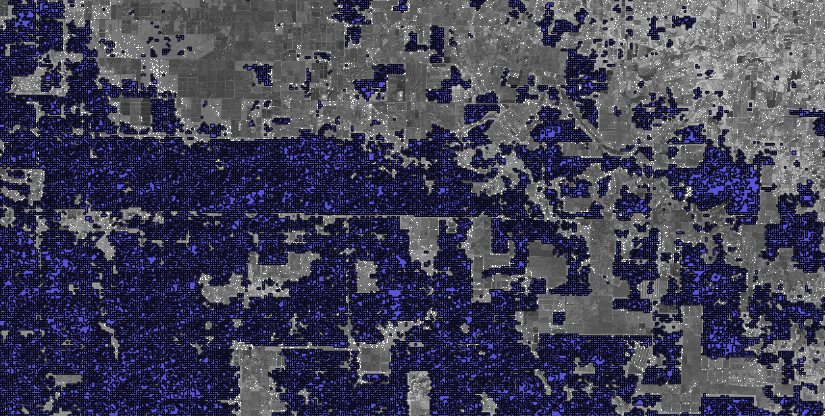
\includegraphics[width=0.8	\textwidth]{./Figures/cap5/mascaraVCF.png}
	\caption{Mascara VCF de 0-30\% sobre NDVI a\~{n}o 2000}
	\label{fig:mascVCf}
\end{figure}
Posteriormente se extrajeron 2000 puntos aleatorios, para muestreo, de la mascara VCF, donde estaran los valores de NDVI..
\begin{figure}[H]
	\centering
	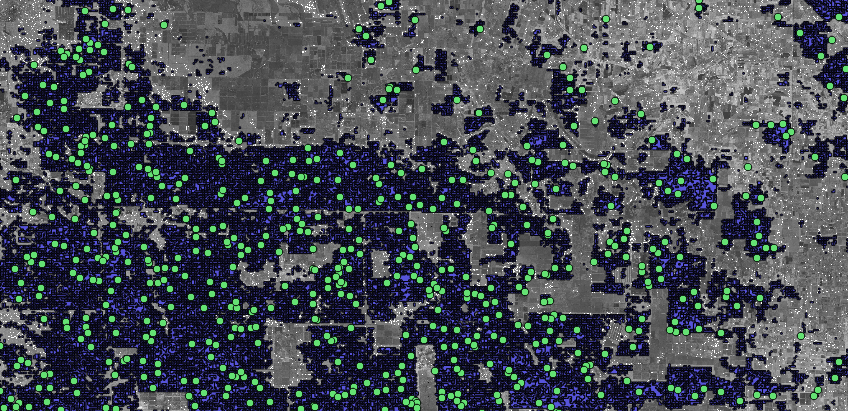
\includegraphics[width=0.8	\textwidth]{./Figures/cap5/vcfAleatorio.png}
	\caption{Puntos aleatorios dentro de la mascara VCF.}
	\label{fig:aleatorioVCf}
\end{figure}
El procedimiento se repite para cada mascara en los distintos rangos. En total se obtiene 5 grupos por cada a\~{n}o estudiado con estad\'isticas ilustrada en la tabla \ref{t:vcfNdvi}.

% Please add the following required packages to your document preamble:
% \usepackage[table,xcdraw]{xcolor}
% If you use beamer only pass "xcolor=table" option, i.e. \documentclass[xcolor=table]{beamer}
\begin{table}[H]
	\centering
	\begin{tabular}{|l|l|l|}
		\hline
		\rowcolor[HTML]{EFEFEF} 
		\multicolumn{3}{|c|}{\cellcolor[HTML]{EFEFEF}\textbf{A\~{n}o 1986}}        \\ \hline
		\rowcolor[HTML]{EFEFEF} 
		\textbf{VCF (\%)} & \textbf{NDVI (Media)} & \textbf{NDVI (Desviaci\'on)} \\ \hline
		50                & 0.356701              & 0.047891                   \\ \hline
		40                & 0.344022              & 0.0507296                  \\ \hline
		30                & 0.337696              & 0.061581                   \\ \hline
		20                & 0.339586              & 0.0632055                  \\ \hline
		10                & 0.335528              & 0.0727573                  \\ \hline
		\rowcolor[HTML]{EFEFEF} 
		\multicolumn{3}{|c|}{\cellcolor[HTML]{EFEFEF}\textbf{A\~{n}o 1990}}        \\ \hline
		\rowcolor[HTML]{EFEFEF} 
		\textbf{VCF (\%)} & \textbf{NDVI (Media)} & \textbf{NDVI (Desviaci\'on)} \\ \hline
		50                & 0.278804              & 0.0631834                  \\ \hline
		40                & 0.264651              & 0.0679451                  \\ \hline
		30                & 0.254145              & 0.0742348                  \\ \hline
		20                & 0.252186              & 0.0759032                  \\ \hline
		10                & 0.251421              & 0.0796667                  \\ \hline
		\rowcolor[HTML]{EFEFEF} 
		\multicolumn{3}{|c|}{\cellcolor[HTML]{EFEFEF}\textbf{A\~{n}o 1990}}        \\ \hline
		\rowcolor[HTML]{EFEFEF} 
		\textbf{VCF (\%)} & \textbf{NDVI (Media)} & \textbf{NDVI (Desviaci\'on)} \\ \hline
		50                & 0.0202133             & 0.0572825                  \\ \hline
		40                & 0.0104289             & 0.0608757                  \\ \hline
		30                & -0.00337075           & 0.066776                   \\ \hline
		20                & -0.00663188           & 0.0695777                  \\ \hline
		10                & -0.0103891            & 0.0757546                  \\ \hline
	\end{tabular}
		\caption{Media y desviaci\'on del muestreo realizado.}
		\label{t:vcfNdvi}
\end{table}

La tabla nos muestra claramente, que la media del NDVI es diferente para cada a\~{n}o, independientemente del porcentaje de vegetaci\'on evaluado. En este caso, no es conveniente tomar la media dentro de un patrón de comportamiento, con el fin de discriminar la vegetaci\'on. Por otro lado, las desviaciones presentan peque\~{n}as diferencias no considerables, lo cual es debido, a que el \'area foliar (hojas) en la vegetaci\'on posee diferente vigor en cada estaci\'on o condici\'on clim\'atica, al momento de ser capturado su reflectividad por sensores del sat\'elite.\\~\\
De esta manera se realiza un promedio entre todas las desviaciones, quedando como valor constante en la umbralizaci\'on de vegetaci\'on \ref{sec:uvegetacion}$ \sigma_{ndvi} = 0.0658242733 $.
\subsection{Estimaci\'on de p\'erdida de carbono forestal}
Gracias al Mapa Global de Carbono \ref{sec:saatchiMapa} es posible analizar la relaci\'on que posee con los indices de vegetaci\'on. El mapa corresponde a fechas cercanas al a\~{n}o 2000, por lo que para el estudio, se obtuvieron im\'agenes Landsat del a\~{n}o 2003 para el calculo de NDVI. Posteriormente se generaron 240 puntos aleatorios dentro \'areas que correspond\'ian a vegetaci\'on.
\begin{figure}[H]
	\centering
	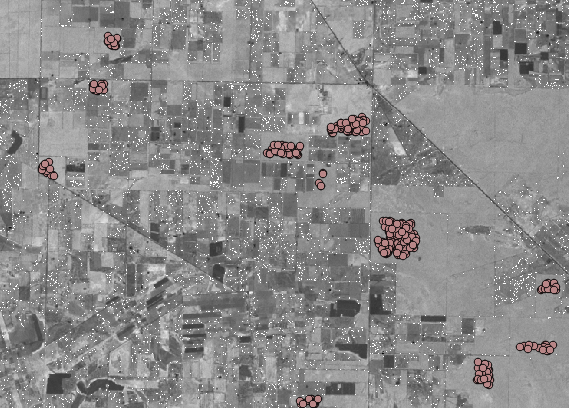
\includegraphics[width=0.8	\textwidth]{./Figures/cap5/carbNdvi.png}
	\caption{Puntos aleatorios.}
	\label{fig:aleatorioCrb}
\end{figure}
Estos puntos fueron generados para interceptar en ellos, los NDVI y ton C/ha en el espacio geográfico. De esa manera nos permiti\'o realizar un an\'alisis de regresi\'on. Inicialmente se hallo una ecuaci\'on lineal, donde el coeficiente de determinaci\'on fue moderado ($ r^{2}=0.509125 $).
\begin{figure}[H]
	\centering
	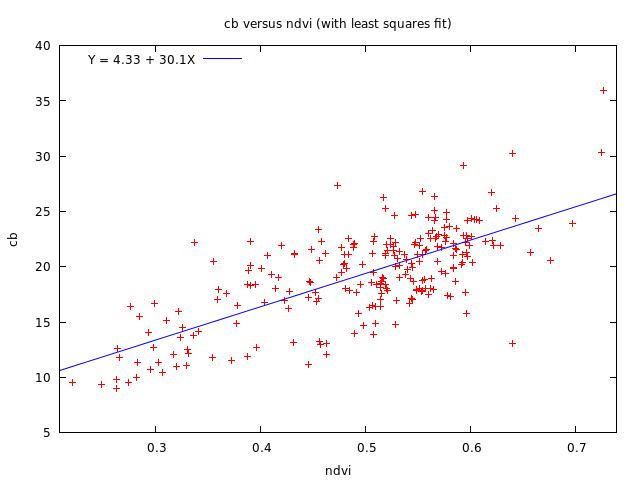
\includegraphics[width=0.8	\textwidth]{./Figures/cap4/ndviCarb.png}
	\caption{Regresi\'on Lineal. $ X=NDVI, Y=TonC/ha $}
	\label{fig:linealCar}
\end{figure}
En la misma forma se construyo una ecuaci\'on cuadr\'atica, pero el coeficiente de determinaci\'on era semejante al lineal $ r^{2}=0.509273 $.
\begin{figure}[H]
	\centering
	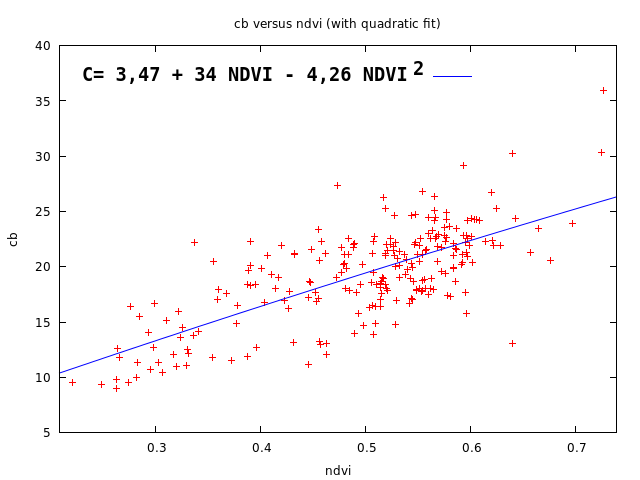
\includegraphics[width=0.8	\textwidth]{./Figures/cap4/ndvCarCuadratico.png}
	\caption{Regresi\'on cuadr\'atica. $ X=NDVI, Y=TonC/ha $}
	\label{fig:cuaCar}
\end{figure}
De esta manera, se opta por la ecuaci\'on lineal para el calculo de carbono en funci\'on al NDVI:
		\begin{equation}
		C=4,33+30,1 NDVI
		\end{equation} 
Siendo $ C $ toneladas de carbono por hect\'area.

\subsection{Prueba experimental} 
Con el prop\'osito de evaluar la calidad en la detecci\'on de cambio, se obtuvieron las im\'agenes que fueron utilizadas en la elaboraci\'on del Paraguay Forest Change Product \ref{sec:fcc}. Dichas im\'agenes corresponden a la fecha 1-26-1992	del sat\'elite Landsat-5 y 8-17-1999 del satelite Landsat-7, con path-row 228-76 del WRS-2 correspondiente al \'area del caso de estudio.\\~\\
Se delimitaron 3 tipos de \'areas, donde cada uno representa un sector las \'areas urbana, rural y h\'umeda. Esto es con el fin de evaluar la detecci\'on en diferentes condiciones o usos del suelo.
\begin{itemize}
	\item \textbf{\'Area Urbana:} zona de aglomeramiento y mayor densidad poblacional. Existe predominio  de actividades econ\'omicas no agropecuarias, sumado a la poblaci\'on total. 
	\item \textbf{\'Area Rural:} se caracteriza por la inmensidad de espacios verdes que la componen y que por esta razón est\'a destinada y es utilizada para la realizaci\'on de actividades agropecuarias y agro-industriales, entre otras.
	\item \textbf{\'Area H\'umeda:}	zona de tierras, generalmente planas, cuya superficie se inunda de manera permanente o intermitente-mente.
\end{itemize}
\begin{figure}[H]
	\centering
	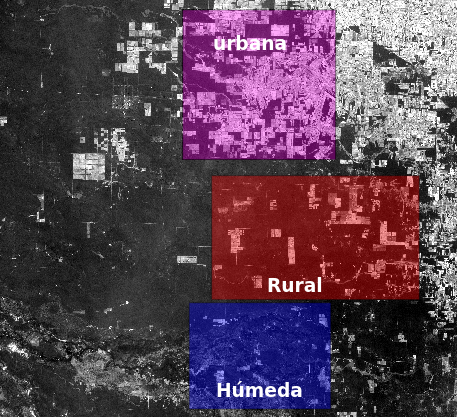
\includegraphics[width=0.8	\textwidth]{./Figures/cap5/zonas.png}
	\caption{Sectores de estudio.}
	\label{fig:zonasEva}
\end{figure}
\begin{table}[H]
	\centering
	\begin{tabular}{|l|l|l|l|l|l|l|}
		\hline
		\rowcolor[HTML]{EFEFEF} 
		\textbf{Sector} & \textbf{xMin} & \textbf{yMin} & \textbf{xMax} & \textbf{yMax} & \textbf{Has.} & \textbf{Km.} \\ \hline
		Urbano          & 748797.48     & -2532113.76   & 799869.96     & -2482116.50 & 255348.41 & 202.13   \\ \hline
		Rural           & 758474.37     & -2578885.40   & 827825.42     & -2537489.81 & 287082.72 & 221.49  \\ \hline
		Húmedo          & 750947.90     & -2615442.54   & 798257.14     & -2579960.61 & 167862.32 & 165.58	  \\ \hline
	\end{tabular}
		\caption{Pol\'igono de las \'areas. Sistema de coordenadas UTM Zona 20 K. }
		\label{t:poligonos}
\end{table}
La metodolog\'ia fue implementada como un complemento al Quantum GIS\ref{sec:quantum}, de manera a poder realizar las pruebas. 
\begin{figure}[H]
	\centering
	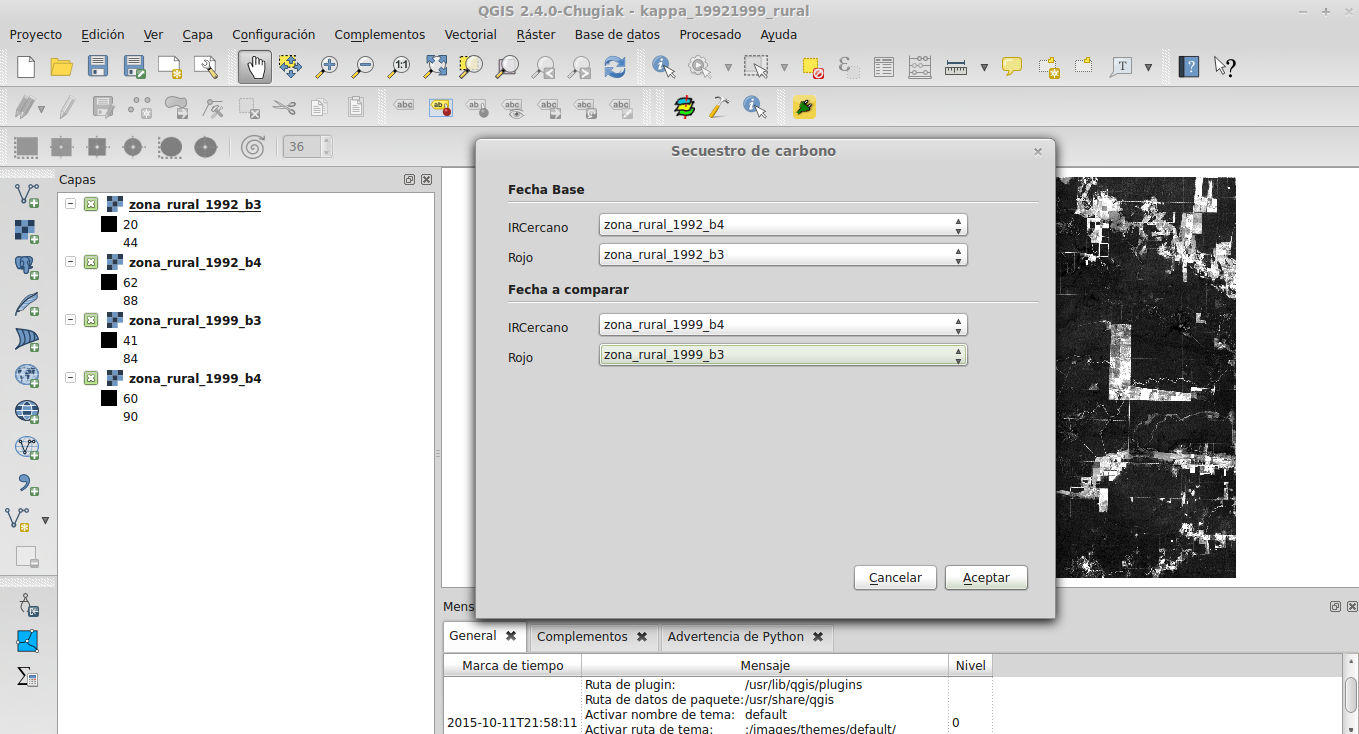
\includegraphics[width=0.8	\textwidth]{./Figures/cap5/qgisCarbono.png}
	\caption{Complemento Quantum GIS.}
	\label{fig:qgisC}
\end{figure}
El proceso de correcci\'on de las im\'agenes satelitales \ref{sec:coorImsat}, debido a que obtuvieron los productos L1T del USGS \ref{sec:landsat}, no fueron implementados por ya poseer el pre-procesamiento de correcci\'on geom\'etrica y radiom\'etrica correspondiente. Esto es beneficioso al estudio en cuanto a costo, por que no es necesario el levantamiento de los puntos de control (GCP) en el terreno para la correcci\'on geom\'etrica espec\'ificamente. La interpolaci\'on espacial fue hecha por un polinomio cuadr\'atico y la radiom\'etrica por el m\'etodo de convoluci\'on cubica.
% Please add the following required packages to your document preamble:
% \usepackage[table,xcdraw]{xcolor}
% If you use beamer only pass "xcolor=table" option, i.e. \documentclass[xcolor=table]{beamer}
\begin{table}[H]
	\centering

	\begin{tabular}{|l|l|l|l|l|}
		\hline
		\rowcolor[HTML]{EFEFEF} 
		\textbf{Sat\'elite} & \textbf{Path-row} & \textbf{Fecha} & \textbf{RMSE} & \textbf{GCP} \\ \hline
		Landsat-5         & 228-76            & 1-26-199       & 4.302         & 108          \\ \hline
		Landsat-7         & 229-76            & 8-17-1999      & 4.066         & 199          \\ \hline
	\end{tabular}
		\caption{RMSE obtenido del meta-dato de cada imagen obtenida.}
		\label{t:rmse}
\end{table}

Se recortaron las bandas de las im\'agenes, infrarroja cercana y roja $ (B4,B3) $, para cada sector y fecha e introducidas como datos de entrada al complemento, ilustraci\'on \ref{fig:qgisC}. A continuaci\'on se muestran los resultados de cada sector con diferentes coeficientes de tolerancia, descripto en la secci\'on \ref{sec:discriminacion}, luego de pasar por el complemento:
\begin{figure}[H]
	\centering
	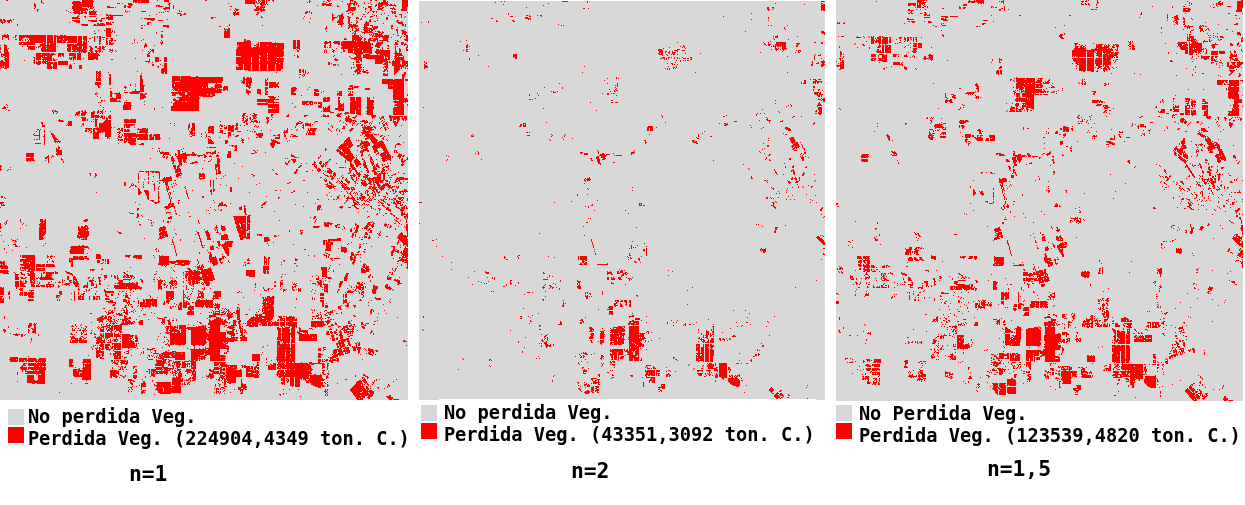
\includegraphics[width=0.8	\textwidth]{./Figures/cap5/res_zona_urbana.png}
	\caption{\'Area Urbana.}
	\label{fig:ubana}
\end{figure}
\begin{figure}[H]
	\centering
	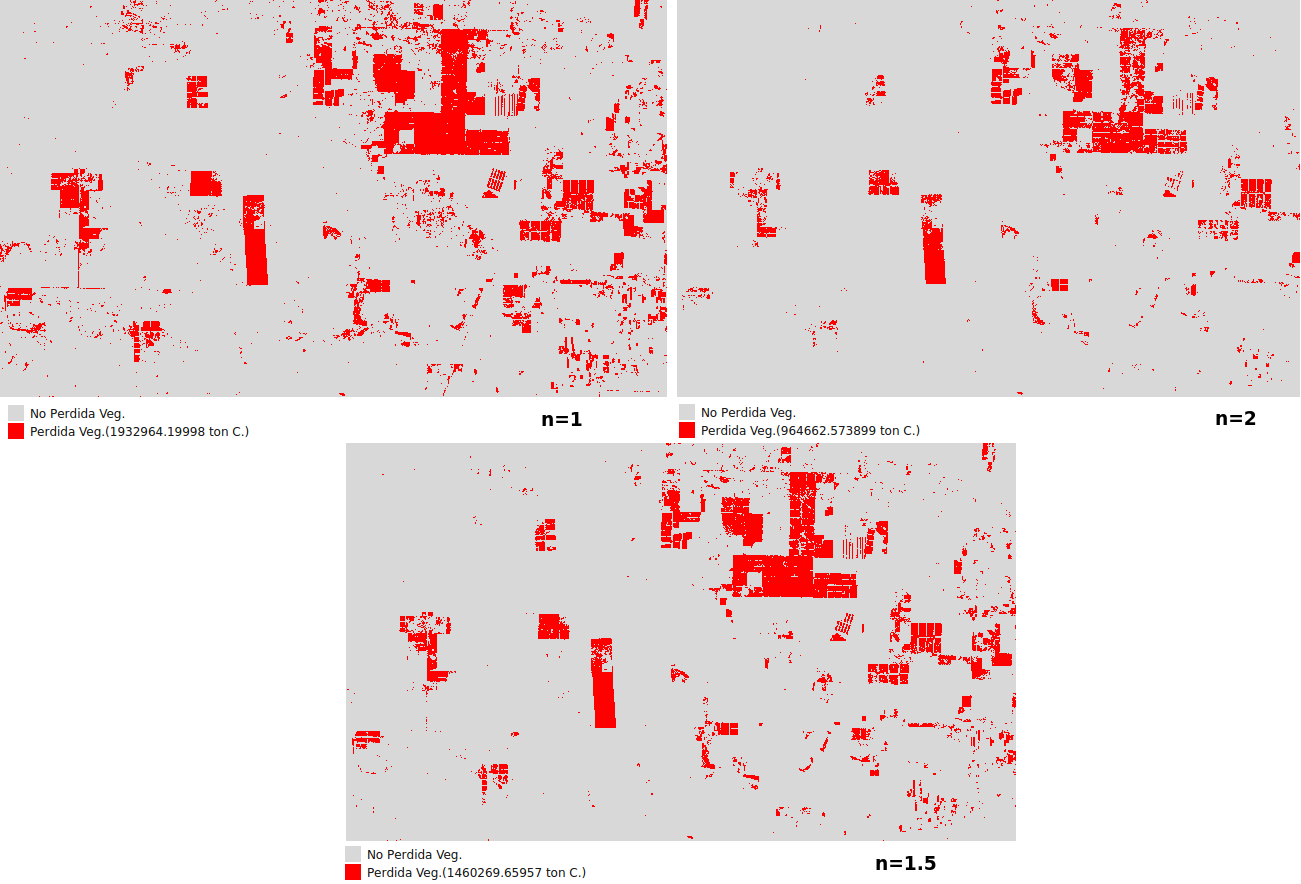
\includegraphics[width=0.8	\textwidth]{./Figures/cap5/res_zona_rural.png}
	\caption{\'Area Rural.}
	\label{fig:rural}
\end{figure}
\begin{figure}[H]
	\centering
	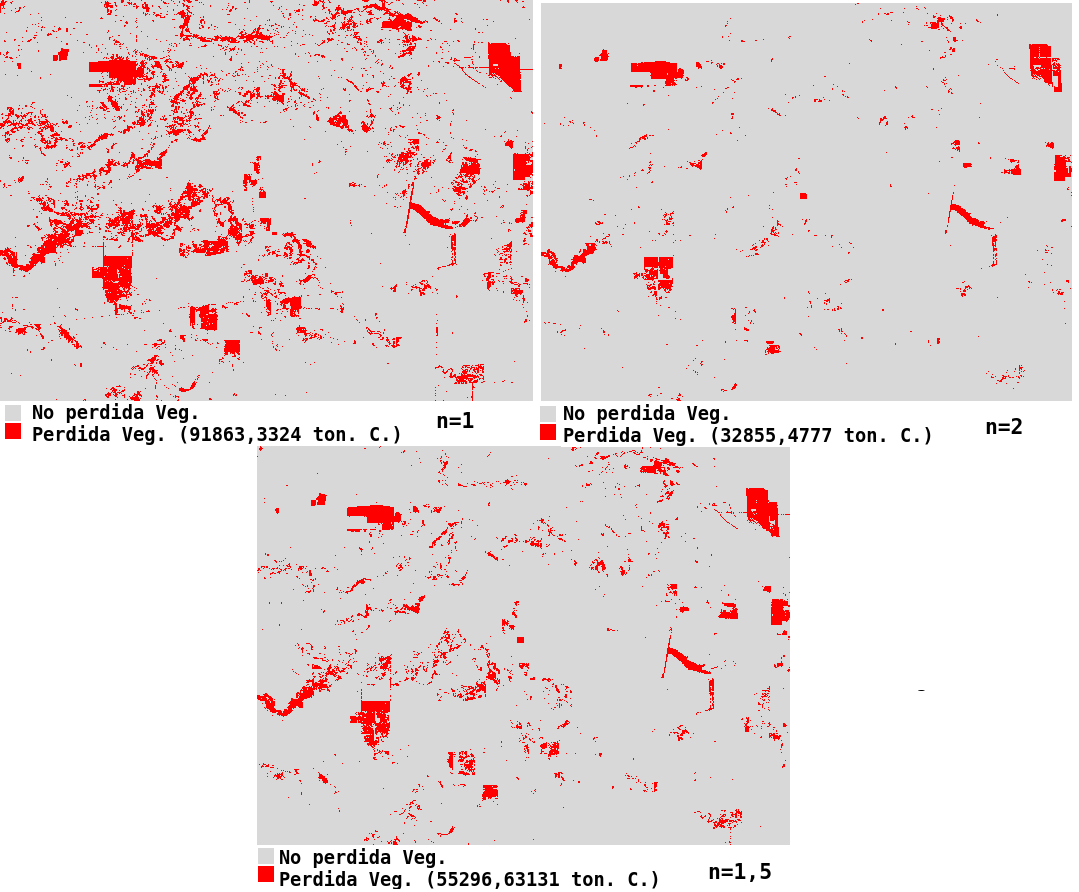
\includegraphics[width=0.8	\textwidth]{./Figures/cap5/res_zona_humeda.png}
	\caption{\'Area H\'umeda.}
	\label{fig:humeda}
\end{figure}

\subsection{Discusi\'on de resultados}
La evaluaci\'on de la calidad en la detecci\'on de perdida forestal fueron hechas con la comparaci\'on del Paraguay Forest Change Produc (PFCP) y los resultados obtenidos por cada sector y coeficiente de tolerancia $ (n) $. El indice kappa y la precision Global nos permitira saber la calidad en los resultados de detecci\'on de cambio.\\~\\
Previamente se realizo una re-clasificaci\'on en la imagen PFCP, ya que en ella refleja varios tipos de bosques y no bosques, por ello se procedi\'o a dejar solo aquellos pixeles que representan perdida de vegetaci\'on en cualquier de los tipos.
\begin{figure}[H]
	\centering
	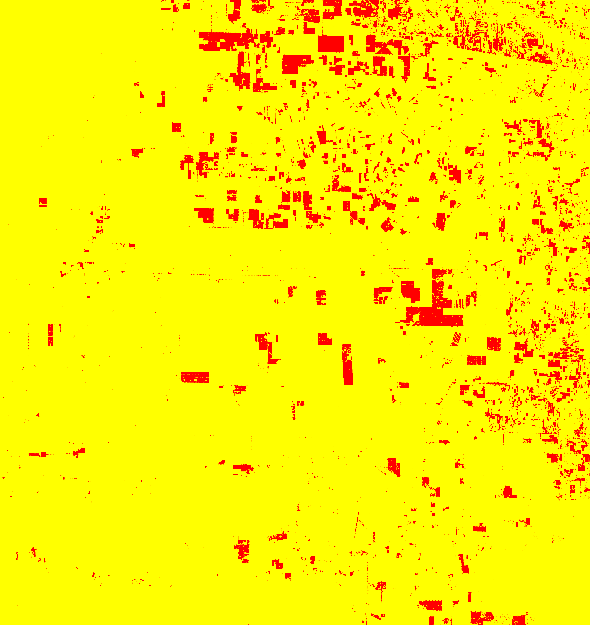
\includegraphics[width=0.8	\textwidth]{./Figures/cap5/pcfp.png}
	\caption{Re-clasificaci\'on de la imagen PFCP. Perdida = 2, Otros=1}
	\label{fig:pfcp}
\end{figure}
Una vez generado la imagen de referencia para la evaluaci\'on, con ayuda de la aplicaci\'on GRASS GIS \ref{sec:grass} se obtuvo los siguientes resultados:
% Please add the following required packages to your document preamble:
% \usepackage[table,xcdraw]{xcolor}
% If you use beamer only pass "xcolor=table" option, i.e. \documentclass[xcolor=table]{beamer}
\begin{table}[H]
	\centering

	\begin{tabular}{|l|l|l|}
		\hline
		\rowcolor[HTML]{EFEFEF} 
		\multicolumn{3}{|l|}{\cellcolor[HTML]{EFEFEF}\textbf{N=1}}   \\ \hline
		\rowcolor[HTML]{EFEFEF} 
		\textbf{\'Area}  & \textbf{Kappa}  & \textbf{Precisi\'on Global} \\ \hline
		Urbano         & 0.476389        & 84.257452                 \\ \hline
		Rural          & 0.65782         & 93.82121                  \\ \hline
		H\'umeda         & 0.301541        & 90.624794                 \\ \hline
		\rowcolor[HTML]{EFEFEF} 
		\multicolumn{3}{|l|}{\cellcolor[HTML]{EFEFEF}\textbf{N=1.5}} \\ \hline
		\rowcolor[HTML]{EFEFEF} 
		\textbf{\'Area}  & \textbf{Kappa}  & \textbf{Precisi\'on Global} \\ \hline
		Urbano         & 0.315273        & 83.514875                 \\ \hline
		Rural          & 0.671753        & 94.899171                 \\ \hline
		H\'umeda         & 0.425555        & 96.693648                 \\ \hline
		\rowcolor[HTML]{EFEFEF} 
		\multicolumn{3}{|l|}{\cellcolor[HTML]{EFEFEF}\textbf{N=2}}   \\ \hline
		\rowcolor[HTML]{EFEFEF} 
		\textbf{\'Area}  & \textbf{Kappa}  & \textbf{Precisi\'on Global} \\ \hline
		Urbano         & 0.09368         & 81.642457                 \\ \hline
		Rural          & 0.570687        & 94.33648                  \\ \hline
		H\'umeda         & 0.425555        & 96.693648                 \\ \hline
	\end{tabular}
		\caption{Coeficiente Kappa y precisi\'on Global obtenidos.}
		\label{t:kappaGa}
\end{table}

En la figura \ref{fig:kappaGrafico}, podemos observar que los coeficientes kappas en todos los $ n  $ son mejores para zonas rurales, variando en resultados moderados y considerables. Seguido por zonas h\'umedas, donde $ n=1 $ se obtienen resultados aceptables a diferencia de las dem\'as que son moderadas. Por ultimo las zonas urbanos son las que presentan gran variaci\'on entre los coeficientes hallados para el, debiendo implementar tolerancia baja $(n=1)$, al modelo de detecci\'on, para obtener resultados moderados. Los coeficientes son interpretados seg\'un la tabla \ref{t:kappaTable}.
\begin{figure}[H]
	\centering
	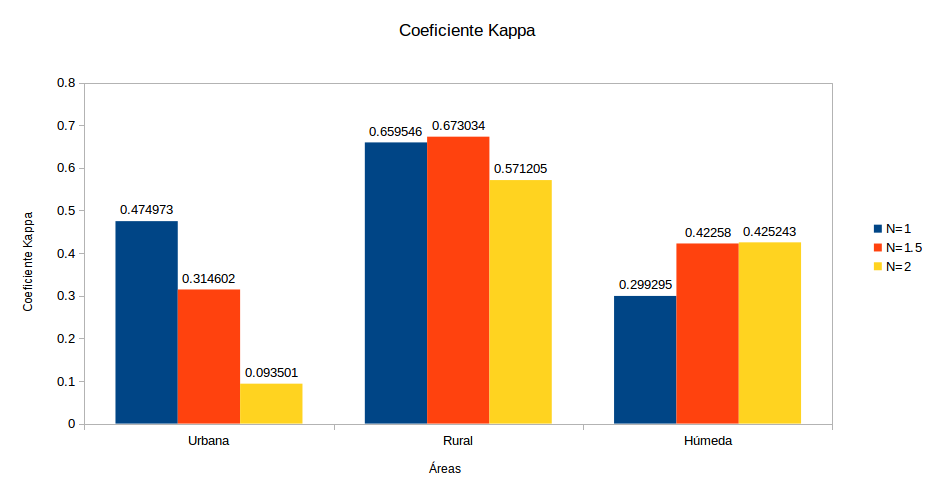
\includegraphics[width=0.8	\textwidth]{./Figures/cap5/kappaGrafico.png}
	\caption{Coeficiente Kappa por cada \'Area y tolerancia.}
	\label{fig:kappaGrafico}
\end{figure}


La precisi\'on global, seg\'un la ilustraci\'on \ref{fig:gaGrafico}, nos dice que el mejor resultado fue en la zona h\'umeda $ (n=2) $ bajando el porcentaje para los dem\'as tolerancias. Pero en zonas rurales obtenemos porcentajes parejos y elevados para cualquier $ n $. Tanto para zonas h\'umedas y rurales seg\'un Jensen \cite{jensen1981urban} son \'optimos por sobrepasar el 85\%. Las zonas urbanas se encuentran entre 81\% - 85\% proximos al umbral, lo que los deja sin ning\'un resultado satisfactorio.
\begin{figure}[H]
	\centering
	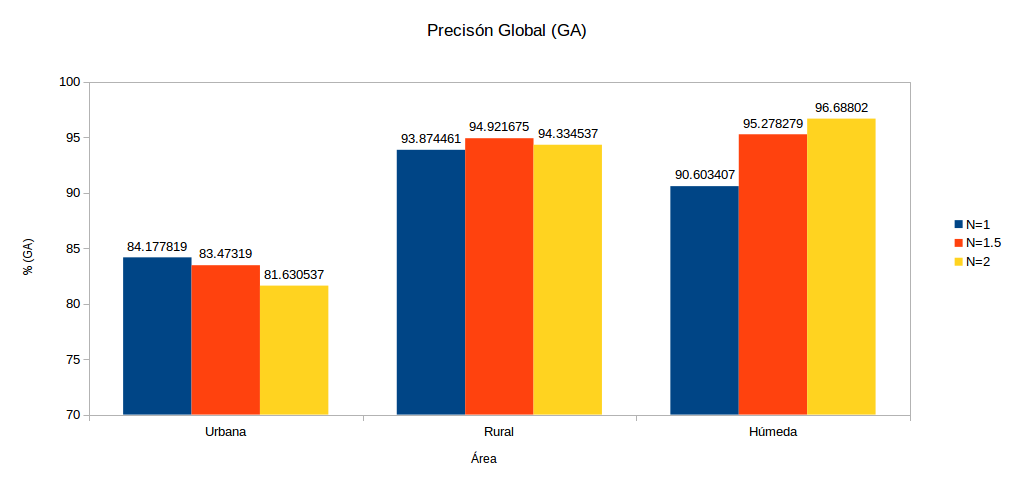
\includegraphics[width=0.8	\textwidth]{./Figures/cap5/gaGrafico.png}
	\caption{GA por cada \'Area y tolerancia.}
	\label{fig:gaGrafico}
\end{figure}

\subsection{Dificultades encontradas} 
Unas de las principales dificultades encontradas fueron en el proceso de correcci\'on geom\'etrica, debido a que es necesario ir al terreno para el levantamiento de puntos de control, sino se utilizan las im\'agenes Landsat prove\'idas por USGS \ref{sec:landsat}. Otro punto considerable a lo que se refiere a dificultad, es que las im\'agenes Landsat presentan un porcentaje de nubosidad, por lo que requerir\'a un pre-procesamiento que permita su utilizaci\'on en el an\'alisis.\\~\\

Habiendo evaluado los resultados en base a los objetivos propuestos, en el siguiente y \'ultimo cap\'itulo se exponen las conclusiones de este trabajo  y finalmente trabajos futuros que puedan dar continuidad a este trabajo final de grado.